% This text is Free and open Open Source.
% It may be used only for academic purpose
% May, 2012
% Author: Seshagiri Prabhu
% Amrita Vishwa Vidyapeethm 
% seshagiriprabhu@gmail.com
% www.seshagiriprabhu.wordpress.com

\documentclass[12pt]{beamer}
\usetheme{Oxygen}
\usepackage{thumbpdf}
\usepackage{wasysym}
\usepackage{ucs}
\usepackage[utf8]{inputenc}
\usepackage{pgf,pgfarrows,pgfnodes,pgfautomata,pgfheaps,pgfshade}
\usepackage{verbatim}
\usepackage{listings}
\usepackage{courier}
\usepackage{caption}
\usepackage{multicol}
\usepackage{verbatim} 
\usepackage{upquote}
%\usepackage{graphics}
% \usepackage[pdftex]{color,graphicx}
\usepackage{latexsym}
\usepackage{hyperref}
\usepackage{xcolor}

\lstset{
  	language=C,
    basicstyle=\ttfamily\footnotesize,
    frame=shadowbox,
    tabsize=4,
    breaklines=true,
    rulecolor=\color{black},
    rulesepcolor=\color{gray},
}

\pdfinfo
{
  	/Title       (Stack Frames)
  	/Creator     (Seshagiri Prabhu)
  	/Author      (TeX)
}

\title{CTF Workshop}
\subtitle{}
\author{Seshagiri Prabhu}
\institute[Amrita Vishwa Vidyapeetham] % (optional)
{
  	\begin{center}
   	\begin{large}
	    Day 3\\
   	\end{large}
    	Amrita Vishwa Vidyapeetham\\
  		Amritapuri
  	\end{center}
}

\begin{document}
\frame{\titlepage}
\section*{}
\begin{frame}
	\frametitle{Outline}
  	\tableofcontents[section=1,hidesubsections]
\end{frame}


%%%%%%%%%%%%%%%%%%%%%%%%%%%%%%%%%%%%%%%%%
%%%%%%%%%% Content starts here %%%%%%%%%%
%%%%%%%%%%%%%%%%%%%%%%%%%%%%%%%%%%%%%%%%%


\section{The Stack}
	\begin{frame}{}
	\frametitle{The stack}
			\begin{itemize}
	    		\item The stack grows towards lower memory addresses
	    		\item The stack pointer (\%esp) points to the top of the stack (the
lowest valid address)
				\begin{center}
					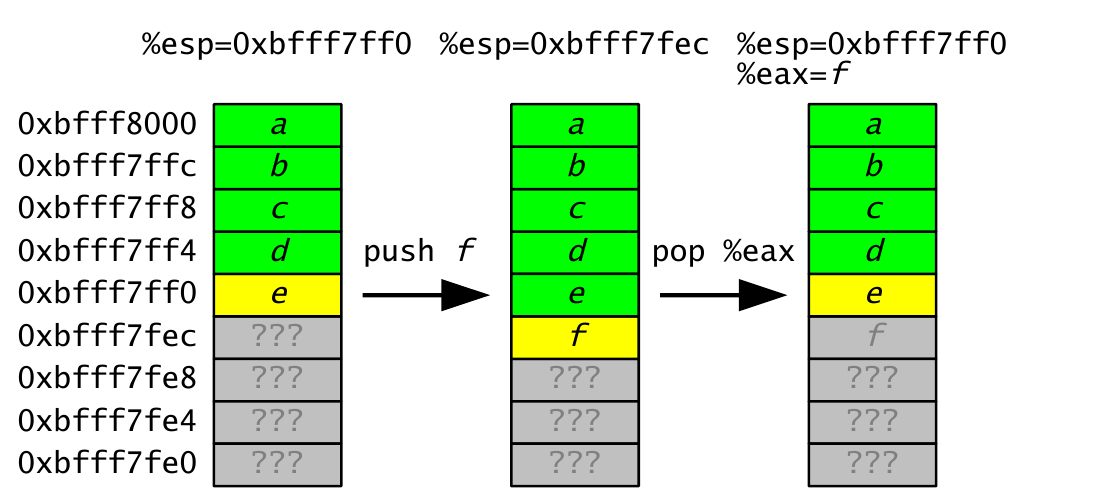
\includegraphics[scale=0.24]{images/stack1.png} 
				\end{center}
  		\end{itemize}	
  	\end{frame}
 	
	\begin{frame}{Frames \& Func invocation I}
  		\frametitle{Frames \& function call I}
  		\begin{itemize}
  		\item The stack is composed of frames
  		\item Frames are pushed on the stack as a consequence of function calls (function prologue)
  		\item The address of the current frame is stored in the Frame Pointer (FP) register
  		\begin{itemize}
		\item On Intel architectures \texttt{\%ebp} is used
  		\end{itemize}
		\item Each frame contains
		\begin{itemize}
		\item The function’s actual parameters
		\item The return address to jump to at the end of the function
		\item The pointer to the previous frame
		\item Function’s local variables
		\end{itemize}
		\item Compiler optimization may eliminate stack frames
		\end{itemize}
	\end{frame}
	
 	\begin{frame}{}
 		\frametitle{Frames \& Func call II}
 		\small
		\lstinputlisting[]{code/code1.c}
		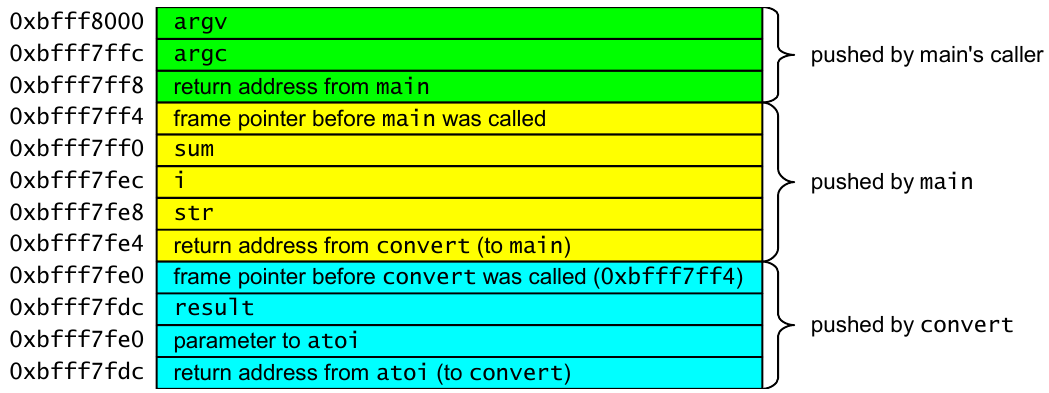
\includegraphics[scale=0.2]{images/stack2.png} 
 	\end{frame}
 	
	\begin{frame}{}
		\frametitle{Function prologue}
		\begin{itemize}
			\item Before calling a function the caller prepares the parameters by 
			either setting specific registers or by pushing them on the stack
			\item The prologue of the called function
			\begin{itemize}
				\item Pushes the current base pointer on the stack
				\item Sets the base pointer to be the current stack pointer
				\item Moves the stack pointer onward to make room for local variables \\
				\texttt{push \%ebp} \\
				\texttt{mov \%esp, \%ebp} \\
				\texttt{sub \$n, \%esp} \\
			\end{itemize}
		\end{itemize}
	\end{frame}	 
	
	\begin{frame}
		\frametitle{Function Epilogue}
		\begin{itemize}
			\item The epilogue of the called function
			\begin{itemize}
				\item Saves the results (if any) in the \texttt{\%eax} register
				\item Stores the base pointer into the stack pointer (deletes the current
				 stack frame)
				\item Pops a value from the stack, restoring the saved base pointer
				\item Executes a \texttt{ret}
			\end{itemize}
			\item The second and third operations are equivalent to the \texttt{LEAVE} opcode
		\end{itemize}
	\end{frame}
	
	\begin{frame}[fragile]
	\frametitle{Example}
	\small
	\lstinputlisting[c]{code/code2}
	\lstinputlisting[asm]{code/code3}	
	\end{frame}
	
	
\section{Process}
	\begin{frame}
		\frametitle{A Program's Life}
		\begin{itemize}
			\item Design
			\item Development, usually in a high-level language
			\item Compilation/translation into binary form (object form) by a compiler or assembler
			\item Programs in interpreted languages are translated into an intermediate format
			\item Execution by a process 
			\item Termination
		\end{itemize}
	\end{frame}
	
	\begin{frame}
		\frametitle{Objects}
		\begin{itemize}
			\item Object files include applications and libraries
			\item Object files in general contain:
			\begin{itemize}
				\item The code, in binary format
				\item Relocation information about things that need to be fixed once
						the code and the data are loaded into memory
				\item Information about the symbols defined by the object file and
						the symbols that are imported from different objects
				\item Optionally, debugging information
			\end{itemize}
		\end{itemize}
	\end{frame}
	
	\begin{frame}
		\frametitle{Linking}
		\begin{itemize}
			\item Linking is the process of resolving references that a program
				has to external objects (variables, functions)
			\item Static linking is performed at compile-time
			\item Dynamic linking is performed at run-time
		\end{itemize}
	\end{frame}
	
	\begin{frame}
		\frametitle{The ELF File Format I}
		\begin{itemize}
			\item The Executable and Linkable Format (ELF) is one of the most used binary object formats
			\item ELF files are of three types
			\begin{itemize}
				\item relocatable: need to be fixed by the linker before being executed
				\item executable: ready for execution (all symbols have been 
						resolved with the exception of those related to shared libs)
				\item shared objects: shared libraries with the appropriate linking information
			\end{itemize}
		\end{itemize}
	\end{frame}
	
	\begin{frame}
		\frametitle{The ELF File Format II}
		\begin{itemize}
			\item A program is seen as a collection of segments by the loader
			and as a collection of sections by the compiler/linker
			\item A segment is usually made of several sections
			\item The segment structure is defined in the Program Header Table
			\item The section structure is defined in the Section Header Table
		\end{itemize}
	\end{frame}
	
	\begin{frame}
		\frametitle{Process Structure}
		\begin{itemize}
			\small
			\item Environment/Argument section
			\begin{itemize}
				\item Used for environment data
				\item Used for the command line data
			\end{itemize}
			\item Stack section
			\begin{itemize}
				\item Used for local parameters
				\item Used for saving the processor status
			\end{itemize}
			\item Heap section
			\begin{itemize}
				\item Used for dynamically allocated data
			\end{itemize}
			\item Data section (Static/global vars)
			\begin{itemize}
				\item nitialized variables (.data)
				\item Uninitialized variables (.bss)
			\end{itemize}
			\item Code/Text section (.text)
			\begin{itemize}
				\item Usually marked read-only
				\item Modifications causes segfaults
			\end{itemize}
		\end{itemize}
	\end{frame}		
	
	\begin{frame}
		\frametitle{PLT and GOT}
		\begin{itemize}
			\small
			\item When a shared library function is called by a program the
				address called is an entry in the Procedure Linking Table (PLT)
			\item The address contains an indirect jump to the addresses
				contained in variables stored in the Global Offset Table
			\item The first time a function is called, the GOT address is a jump
				back to the PLT, where the code to invoke the linker is called
			\item The linker does its magic and updates the GOT entry, so next
				time the function is called it can be directly invoked
			\item The PLT is read-only, but the GOT is not...
				\begin{itemize}
					\item By overwriting the contents of a GOT entry it is possible to	
					jump to arbitrary locations
				\end{itemize}
		\end{itemize}
	\end{frame}
	\begin{frame}
  	\frametitle{}
  	\framesubtitle{For further reference}
  	\begin{thebibliography}{10}

  	\beamertemplatearticlebibitems

  	\bibitem{beamer-homepage}
	  	\begin{block}{The examples and slides}
        	\newblock{\url{https://bitbucket.org/seshagiriprabhu/binary-exploitation-and-buffer-overflow}}
	  	\end{block}
  	\end{thebibliography}
\end{frame}

\frame{
  	\vspace{2cm}
  	{\huge Questions ?}

  	\vspace{3cm}
  	\begin{flushright}
        Seshagiri Prabhu\\
	    \structure{\footnotesize{seshagiriprabhu@gmail.com}}
  	\end{flushright}
}
\end{document}